\documentclass[student, noshadow, lsr, english, aspectratio=169, t]{ITR_LSR_slides}

\setbeamertemplate{frametitle}{%
  \vspace{0.3cm}% Space between top edge and title
  \if@center
    \begin{centering}
      \textbf{\vphantom{Sp}\insertframetitle\vphantom{Sp}}
      \par
    \end{centering}
  \else
    \textbf{\vphantom{Sp}\insertframetitle\vphantom{Sp}}
    \par
  \fi
  \vspace{0.3cm}% Space between title and content
}

% Add top margin to frames without titles
\addtobeamertemplate{frame begin}{%
  \ifx\insertframetitle\@empty
    \vspace{0.8cm}% Space at top of frames without titles
  \fi
}{}

\addbibresource{ref.bib}
\graphicspath{{pics/}{logos/}}

\title{Analysis and Control of Time-Varying and Perturbed Systems}
\presenter{Keno Bürger}
\typeofpres{Advanced Nonlinear Control}

\usepackage{multirow}
\usepackage{graphicx}
\usepackage[T1]{fontenc}
\usepackage{lmodern}
\usepackage{tabularx}
\usepackage{enumitem}
\usepackage{adjustbox}
\usepackage{array}
\usepackage{booktabs}
\usepackage{makecell}

\begin{document}

\begin{frame}
    \titlepage
\end{frame}


%%%%%%%%%%%%%%%%%%%%%%%%%%%%%%%%%%%%%%%%%%%%%%%%%%%%%%
\section{Introduction}

\begin{frame}
    \frametitle{Main Objective}

    \textbf{Based on:}
    \begin{itemize}
        \item \textit{Nonlinear Control} (Ch. 4): Time-varying and perturbed systems
        \item \textit{Nonlinear Systems} (Ch. 9, 11.5): Stability under perturbations
    \end{itemize}
	\vspace{0.5cm}
    \textbf{Objective:}
    \begin{itemize}
        \item Analyze stability under \textbf{vanishing perturbations} using comparison functions
        \item Study ultimate boundedness for systems with \textbf{non-vanishing perturbations}
        \item Apply Lyapunov-based methods for robust analysis of nonlinear, time-varying systems
        \item Formulate practical and broadly applicable stability conditions
    \end{itemize}
\end{frame}

\begin{frame}
	\frametitle{Lyapunov Theory for Time-Varying Systems}
	% \begin{itemize}
	% 	\item Definition of Uniform, Asymptotic and exponential stability \cite{muennighoff_s1_2025}
	% 	\item Application of Lyapunov Stability Theorems
	% \end{itemize}
	\textbf{Assumptions:}
	\begin{itemize}
		\item Origin $x=0$ is an equilibrium point
		\item Lyapunov function $V(t,x)$ is continuously differentialbe, positive definite and radially unbounded
		\item Derivative of Lyapunov function is negative definite
	\end{itemize}
	\vspace{0.5cm}
	\textbf{Globally uniformly exponentially stable:}
	\begin{align*}
		\exists\, c_i, \alpha > 0: & \; c_1\left\|x\right\|^\alpha \leq V(t,x) \leq c_2\left\|x\right\|^\alpha  \\
		& \dot{V}(t,x) \leq -c_3\|x\|^\alpha
	\end{align*}
\end{frame}

\begin{frame}
	\frametitle{Boundedness and Ultimate Boundedness}
	% \begin{itemize}
	% 	\item Differences
	% 	\item Build bridge to non vanishing and vanishing perturbations
	% \end{itemize}
	\begin{figure}
		\centering
		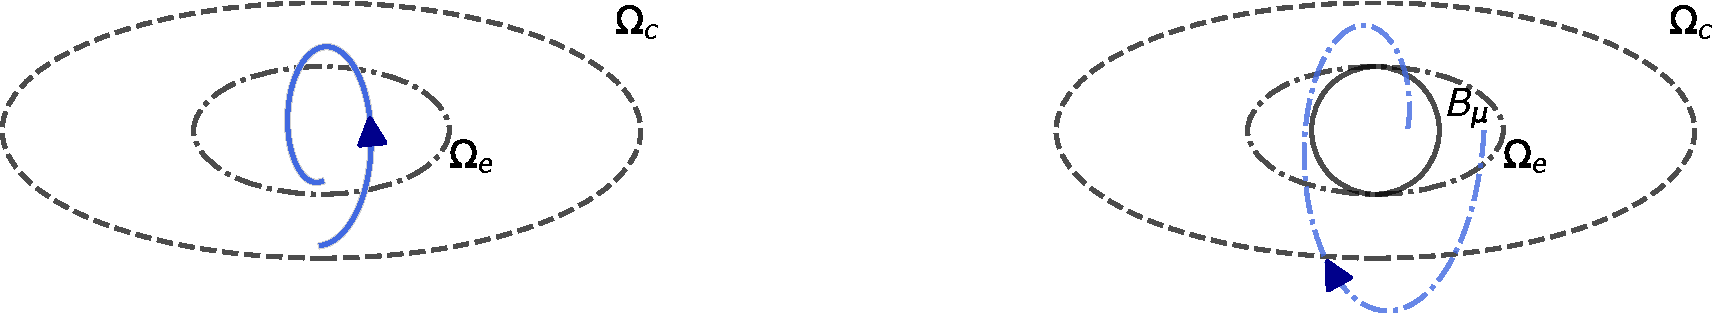
\includegraphics[width=\textwidth]{ultimate_boundedness_rotated.pdf}
		\caption{}
		\label{fig:boundedness_vs_ultimate_boundedness}
	\end{figure}
	\vspace{-1cm}
	\begin{columns}[t,totalwidth=\textwidth]
        \column{0.47\textwidth}
		\textbf{Boundedness:}
		\begin{align*}
			\|x(t_0)\| \leq \alpha \Rightarrow \|x(t)\| \leq \beta,
			\\ c>0, \alpha\in(0,c),\, \beta>0,\,\forall\, t \geq t_0
		\end{align*}

        \column{0.47\textwidth}
		\textbf{Ultimate Boundedness:}
		\begin{align*}
			\|x(t)\| \leq b 
			\\ \forall\, t \geq t_0+T
		\end{align*}
    \end{columns}
\end{frame}

%%%%%%%%%%%%%%%%%%%%%%%%%%%%%%%%%%%%%%%%%%%%%%%%%%%%%
\section{Vanishing Perturbations}
\begin{frame}
	\frametitle{Perturbation Model for Vanishing Perturbation Models}
	\begin{itemize}
		\item Exact Modelling rarley feasible due to modelling errors/external disturbances or parameter drift
		\item $\dot{x}=f(x)+g(x,t)$
		\begin{itemize}
			\item f is locally Lipschitz
			\item g is piecewise continuous in t and locally Lipschitz
			\item generally unknown but bounded
		\end{itemize}
		\item $g(0,t)$ and $g(x,t)=0$ for $t\rightarrow\infty$
	\end{itemize}
\end{frame}


\begin{frame}
	\frametitle{Lyapunov Stability Theorems}
	% \begin{itemize}
	% 	\item Exponential Stability
	% 	\item Highlight challenges with this approach
	% \end{itemize}
	\textbf{Assumptions:}
	\begin{itemize}
		\item Origin $x=0$ is an exponentially stable equilibrium point
		\item Perturbation vanishes
		\item Lyapunov function $V(t,x)$ is continuously differentialbe, positive definite and radially unbounded
	\end{itemize}
	\vspace{0.5cm}
	\textbf{Globally Uniformly Exponentially Stable Equilibrium:}
	\begin{align*}
		\frac{\partial V}{\partial t}+\frac{\partial V}{\partial x}f(x) \leq c_3\|x\|^2 \text{ and }\|\frac{\partial V}{\partial x}\| \leq c_4\|x\|
	\end{align*}
	\begin{align*}
		\|g(x,t)\| \leq \gamma\|x\| \text{ with }0\leq\gamma(t)<\frac{c_3}{c_4}
	\end{align*}

\end{frame}

\begin{frame}
	\frametitle{Comparison Functions}
	% \begin{itemize}
	% 	\item Differences and Benefits of this approach
	% 	\item Corollary 1
	% \end{itemize}
	\textbf{Assumptions:}
	\begin{itemize}
		\item Origin $x=0$ is an exponentially stable equilibrium point
		\item Perturbation vanishes
	\end{itemize}
	\vspace{0.5cm}
	\textbf{Exponential Stability:}
	\begin{align*}
		\|g(x,t)\| \leq \gamma(t)\|x\| \text{ with }\int_{t_0}^{t}\gamma(\tau)d\tau<\epsilon(t-t_o)+\eta
	\end{align*}
	\begin{align*}
		\text{with } \epsilon < \frac{c_1c_3}{c_2c_4}
	\end{align*}
\end{frame}

\begin{frame}
	\frametitle{Example: Linear Time-Varying System}
	% \begin{itemize}
	% 	\item $\dot{x}=[A(T)+B(t)]x$
	% 	\item Lyapunov function $V(t,x)$ is positive definite and derivative negative definite
	% 	\item $g(t,x) = B(t)x \Rightarrow \|g(t,x)\| \leq \|B(t)\| \cdot \|x\| = \gamma(t) \|x\|$
	% 	\item $\int_{t_0}^{t}\gamma(\tau)d\tau<\epsilon(t-t_o)+\eta$
	% 	\item[$\Rightarrow$] Exponetial stability of nominal system is preserved under vanishing perturbations
	% \end{itemize}
	\textbf{Perturbed Linear Time-Varying System:}
	\begin{align*}
		\dot{x}=[A(t)+B(t)]x
	\end{align*}
	\textbf{Assumptions:}
	\begin{itemize}
		\item $A(t)$ is uniformly bounded
		\item Origin of nominal system is uniformly exponentially stable
		\item $B(t) \rightarrow 0$ as $t\rightarrow\infty$
		\item Lyapunov function $V(t,x)$ is positive definite and derivative negative definite
	\end{itemize}
	\begin{align*}
		g(t,x) = B(t)x \Rightarrow \|g(t,x)\| \leq \|B(t)\| \cdot \|x\| = \gamma(t) \|x\|
	\end{align*}
	$\Rightarrow$ Exponential stability of nominal system is preserved under vanishing perturbations
	
\end{frame}

%%%%%%%%%%%%%%%%%%%%%%%%%%%%%%%%%%%%%%%%%%%%%%%%%%%%%
\section{Non-Vanishing Perturbations}

\begin{frame}
	\frametitle{Perturbation Model for Non-Vanishing Perturbations}
	% \begin{itemize}
	% 	\item Impede the system's convergence towards the origin
	% 	\item Analysing the behavior in terms of boundedness/ultimate boundedness
	% 	\item Gurantee that the state will remain within a small neighborhood around the origin
	% \end{itemize}
	\begin{itemize}
        \item $g(t,x)$ does not vanish, persistent input or modeling error
        \item Origin is no longer an equilibrium
        \item Use ultimate boundedness: trajectories enter and remain in a compact set
        \item Stability becomes input-to-state-like (robustness to bounded disturbances)
    \end{itemize}
\end{frame}

\begin{frame}
	\frametitle{Lyapunov Based Conditions for Boundednes}
	% \begin{itemize}
	% 	\item Why only boundedness
	% 	\item Lemma 2 for Ultimate Boundedness
	% \end{itemize}
	\textbf{Assumptions:}
	\begin{itemize}
		\item Origin $x=0$ is an exponentially stable equilibrium point
		\item Non vanishing perturbation
		\item Lyapunov function $V(t,x)$ is continuously differentialbe, positive definite and radially unbounded
		\item Derivative of Lyapunov function is negative definite
		\item Perturbation is bounded
		\begin{align*}
			\|g(x,t)\| \leq \delta<\frac{c_3}{c_4}\sqrt{\frac{c_1}{c_2}}\theta r, \text{ with } \in(0,1), r>0
		\end{align*}
	\end{itemize}
\end{frame}

\begin{frame}
	\frametitle{Lyapunov Based Conditions for Boundednes}
	\textbf{Exponetial Stability:} \\
	For all initial conditions $\|x(t_0)|\leq \sqrt{c_1/c_2}r$
	\begin{align*}
		\|x(t)\| \leq ke^{-\gamma(t-t_0)}\|x(t_0)\|, t_0 \leq t \leq t_0+T
	\end{align*}
	\begin{align*}
		\|x(t)\| \leq b \forall\, t \geq t_0+T
	\end{align*}
	\begin{align*}
		\text{where } k=\sqrt{\frac{c_2}{c_1}},\,\gamma=\frac{(1-\theta)c_3}{2c_2},\, b=\frac{c_4}{c_3}k\frac{\delta}{\theta}
	\end{align*}
\end{frame}

\begin{frame}
	\frametitle{Example: Non-Vanishing Perturbation in a Nonlinear System}
	\begin{itemize}
		\item As a special case of non-vanishing perturbations
		\item Stability Theorems
		\item Case distinctions
	\end{itemize}
\end{frame}

%%%%%%%%%%%%%%%%%%%%%%%%%%%%%%%%%%%%%%%%%%%%%%%%%%
\section{Summary and Discussion}

\begin{frame}
	\frametitle{Conceptual Links Between Sections}
	\begin{itemize}
        \item \textbf{Lyapunov Functions:} Central in both cases, quantify energy and decay
        \item \textbf{Main Difference:} Convergence to origin vs. convergence to a bounded set
        \item \textbf{Comparison Lemma:} Powerful for estimating solution bounds in both cases
        \item \textbf{Ultimate Boundedness:} Reflects robustness, common in practical control
        \item \textbf{Design Implication:} Small perturbations can be tolerated if decay is fast; persistent ones require constraint-aware design
    \end{itemize}

    \vspace{0.5em}
    \textbf{Takeaway:} Both frameworks enhance system analysis in the presence of uncertainty. Knowing the type of perturbation guides appropriate control strategies.
\end{frame}

\begin{frame}
    \frametitle{Benefits and Drawbacks of Lyapunov-Based Analysis}

    \textbf{Benefits}
    \begin{itemize}
        \item \text{General applicability:} %Works for nonlinear, time-varying, and perturbed systems
        \item \text{Rigorous and systematic:}% Provides sufficient conditions for stability and boundedness
        \item \text{Insightful design tool:} %Helps in controller synthesis and robustness analysis
        \item \text{Comparison lemma:}% Enables practical bounding of trajectories without solving the system
        \item \text{Handles uncertainty:}% Applicable to both modeling errors (vanishing) and disturbances (non-vanishing)
    \end{itemize}

    \textbf{Drawbacks}
    \begin{itemize}
        \item \text{Constructing Lyapunov functions is hard:}% No general method for nonlinear systems
        \item \text{Results are conservative:}% Conditions are sufficient but not necessary
        \item \text{Limited to local regions:}% Stability often guaranteed only locally unless global bounds are proven
        \item \text{Quantitative bounds may be loose:}% Worst-case growth rate assumptions can overestimate the effect of perturbations
    \end{itemize}
\end{frame}



%%%%%%%%%%%%%%%%%%%%%%%%%%%%%%%%%%%%%%%%%%%%%%%%%%%%%
\begin{frame}[allowframebreaks]
    \frametitle{References}
    \nocite{*} 
    \printbibliography[heading=none]
\end{frame}

\end{document}
